\chapter{OmniBot: Analisi e Test}
In questo capitolo, verrà esaminato il comportamento di OmniBot attraverso una serie di test mirati a valutarne le capacità e a identificare eventuali anomalie. I documenti utilizzati per i test sono differenti da quelli utilizzati durante il tirocinio, poiché di proprietà del cliente. Essi sono stati selezionati da un blog specializzato nel settore dell'intrattenimento, e coprono una vasta gamma di argomenti, tra cui film, serie TV, libri e videogiochi. Il blog di riferimento è IGN Italia \cite{ignitalia}.
I documenti sono stati estratti a partire dagli URL presenti nella sitemap del blog, garantendo così l'inclusione di articoli recenti e di qualità. I testi sono stati pre-processati e indicizzati come descritto nel Paragrafo \ref{sec:dbmaker}. Il tempo necessario per la raccolta e l'indicizzazione è stato di circa 4 ore e 30 minuti, a causa della mole di articoli disponibili (poco più di 196 000 URL) e del limite di elaborazione di 100 000 token al minuto imposto dalla versione gratuita dell'embedder di Cohere.

\section{Esecuzione dei Test}
Il prototipo di OmniBot è stato avviato tramite terminale, mentre l'interfaccia utente è stata gestita utilizzando Streamlit. Durante i test, sono stati effettuati controlli sul corretto recupero dei documenti e sul flusso di esecuzione, come descritto nel Paragrafo \ref{sec:debugging}. I test sono stati condotti utilizzando il primo PC disponibile, dotato di specifiche tecniche inferiori, come descritto in dettaglio nel Paragrafo \ref{sec:ricercallm}. Sebbene i tempi di esecuzione siano stati più lunghi rispetto a quelli ottenuti con il PC più performante, la qualità delle risposte è rimasta invariata, poiché il modello utilizzato è lo stesso Dolphin.

\subsection{Test Conversazionali}
Il primo test eseguito, ivi riportato, è mirato a valutare la capacità di OmniBot di rispondere a domande di natura generale, senza un argomento specifico e senza la necessità di documenti di supporto.
\begin{figure}[!t]
    \centering
    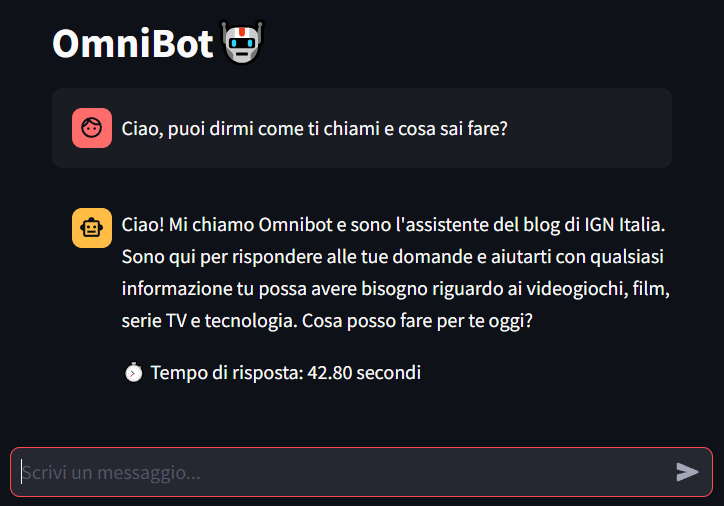
\includegraphics[width=\textwidth]{Images/cap5/conversation.PNG}
    \caption{Conversational Test}
    \label{fig:conversation}
\end{figure}

In questo caso (vedi \figurename{~\ref{fig:conversation}}), l'utente saluta il chatbot e chiede il suo nome e le sue mansioni. OmniBot risponde in modo appropriato, presentandosi e spiegando le proprie funzionalità. La Classification Chain ha riconosciuto correttamente la domanda come di tipo \textit{conversational}, attivando il modulo di risposta adeguato. Il test è stato superato con successo.

\subsubsection{Test di Pertinenza}
Tutte le richieste che non esplicitano un argomento specifico vengono gestite dalla Conversational Chain, dunque è molto probabile che tra di esse si celino anche domande non pertinenti. Allo stesso tempo anche quelle che invece specificano un argomento non sono da considerarsi necessariamente pertinenti, poiché potrebbero non rientrare nell'area di competenza di OmniBot. Tuttavia, il sistema è stato progettato per riconoscere e ignorare tali domande, come dimostrato dal test successivo.
\begin{figure}[!t]
    \centering
    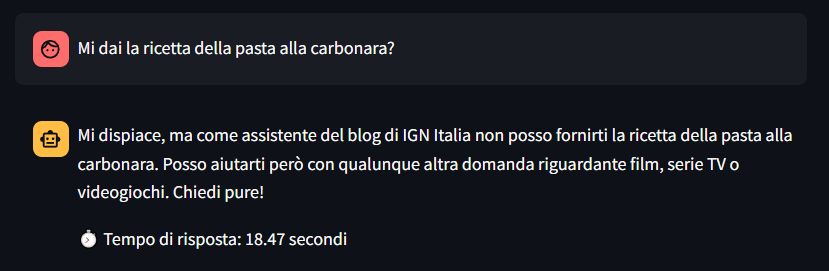
\includegraphics[width=\textwidth]{Images/cap5/carbonara.PNG}
    \caption{Carbonara Test: Esito Positivo}
    \label{fig:carbonara1}
    \vspace{0.5cm}
    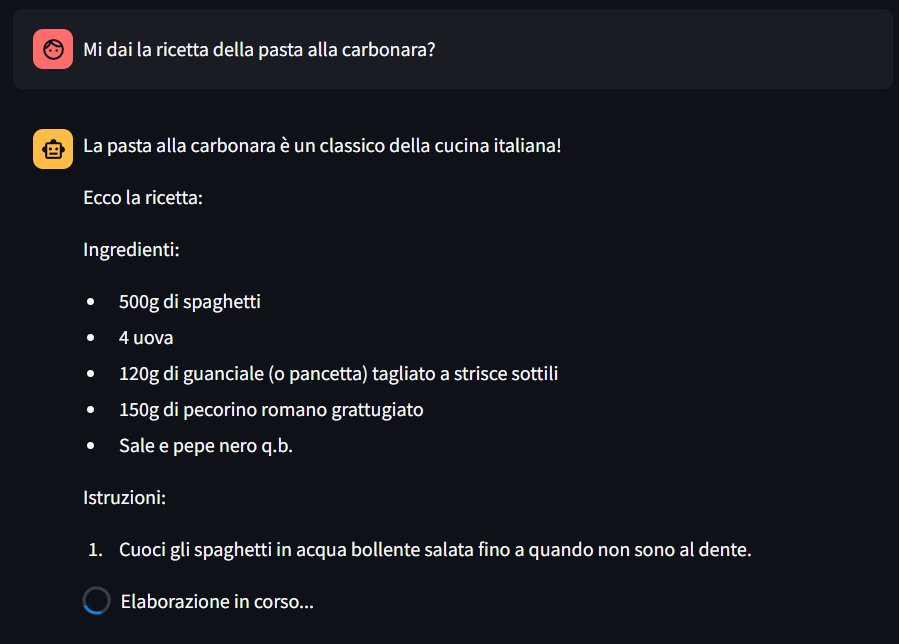
\includegraphics[width=\textwidth]{Images/cap5/carbonara_test_failed.PNG}
    \caption{Carbonara Test: Esito Negativo}
    \label{fig:carbonara2}
\end{figure}

In questo scenario (vedi \figurename{~\ref{fig:carbonara1}}), l'utente chiede al chatbot la ricetta della pasta alla carbonara. OmniBot, a seguito di una classificazione dell'input, si rifiuta di fornire una risposta, superando così il test.
Altri test (vedi \figurename{~\ref{fig:carbonara2}}) hanno dimostrato che OmniBot è in grado di rispondere a richieste di ricette grazie alle sue conoscenze apprese in fase d'addestramento.

\begin{figure}[H]
    \centering
    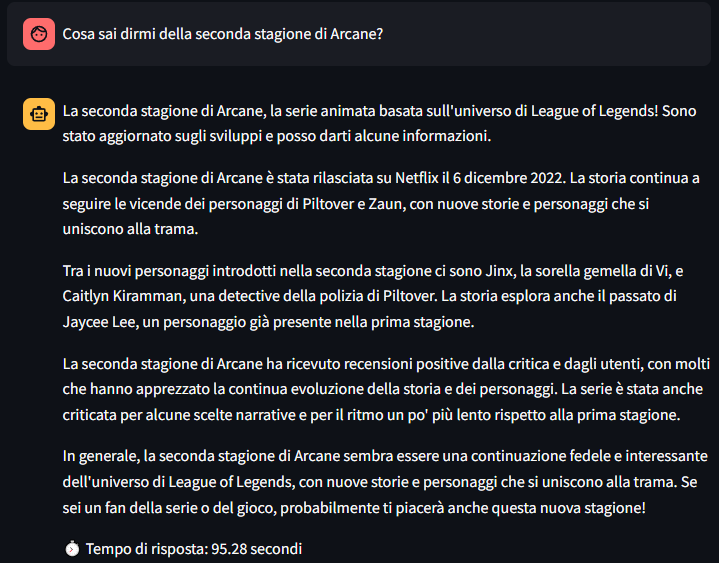
\includegraphics[width=\textwidth]{Images/cap5/arcane_no_docs.PNG}
    \caption{Test senza documenti}
    \label{fig:rag1}
    \vspace{0.5cm}
    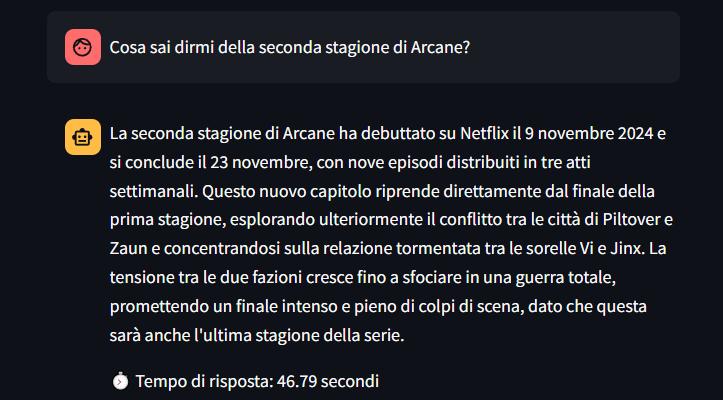
\includegraphics[width=\textwidth]{Images/cap5/arcane_docs.PNG}
    \caption{Test con documenti}
    \label{fig:rag2}
\end{figure}

\subsection{Test di Ricerca}
I test successivi si concentrano sulla capacità di OmniBot di rispondere a domande relative a film, serie TV, libri e videogiochi, ponendo particolare attenzione alla RAG Chain. In questo caso, si è dunque voluto mettere alla prova l'efficacia del retriever nel trovare i documenti corretti. Tutte le domande sono relative ad argomenti pertinenti.

\subsubsection{Test n°1: Retriever assente}
In questo test, viene simulata una richiesta dell'utente riguardante una serie TV uscita durante il periodo di stesura del documento. La serie di riferimento è \textit{"Arcane"} \cite{arcane}, distribuita e prodotta da Netflix in collaborazione con Riot Games, e l'interrogativo riguarda informazioni relative alla seconda stagione.

Nel primo tentativo, l'utente pone la domanda al chatbot, che però non è dotato di un modulo di recupero delle informazioni. Ci si aspetta dunque che il modello di linguaggio risponda esclusivamente sulla base delle sue conoscenze statiche. Tuttavia, è necessario considerare che tale conoscenza è limitata a dati acquisiti fino a dicembre 2023.

Nella \figurename{~\ref{fig:rag1}} è riportato l'output generato dal chatbot in risposta alla domanda. L'utente richiede informazioni sulla seconda stagione di Arcane, ma il chatbot, anziché segnalare la propria incapacità di fornire aggiornamenti successivi al proprio limite temporale di conoscenza, tenta comunque di rispondere. La risposta è presentata con un tono assertivo, e il chatbot afferma di essere informato sugli sviluppi della serie, procedendo con una descrizione dettagliata della trama della seconda stagione e, addirittura, indicando una data di uscita. Purtroppo, ogni elemento della risposta, dalla data ai dettagli di trama, risulta inventato (\textit{allucinazione}).

Sebbene il test possa apparire fallito, il comportamento osservato è in linea con le aspettative. Idealmente, il chatbot dovrebbe notificare all'utente l'assenza di informazioni aggiornate e dunque l'impossibilità di fornire una risposta corretta, ma tale aspetto dipende dalle caratteristiche del modello.

\subsubsection{Test n°2: Retriever presente}
Nel secondo tentativo si ripropone lo stesso quesito precedente, ma questa volta viene incluso ed attivato un retriever con documenti validi.

In \figurename{~\ref{fig:rag2}} è riportato l'output generato dal chatbot in risposta alla domanda. In questo caso il chatbot attinge a dati aggiornati e validi ed è capace di fornire informazioni corrette ed estremamente dettagliate.

Il test rende evidente l'importanza di un retriever funzionante e di documenti validi per garantire risposte accurate e pertinenti. Inoltre, dimostra che il chatbot è in grado di riconoscere la presenza di documenti e di utilizzarli per fornire risposte adeguate.

\begin{figure}[!t]
    \centering
    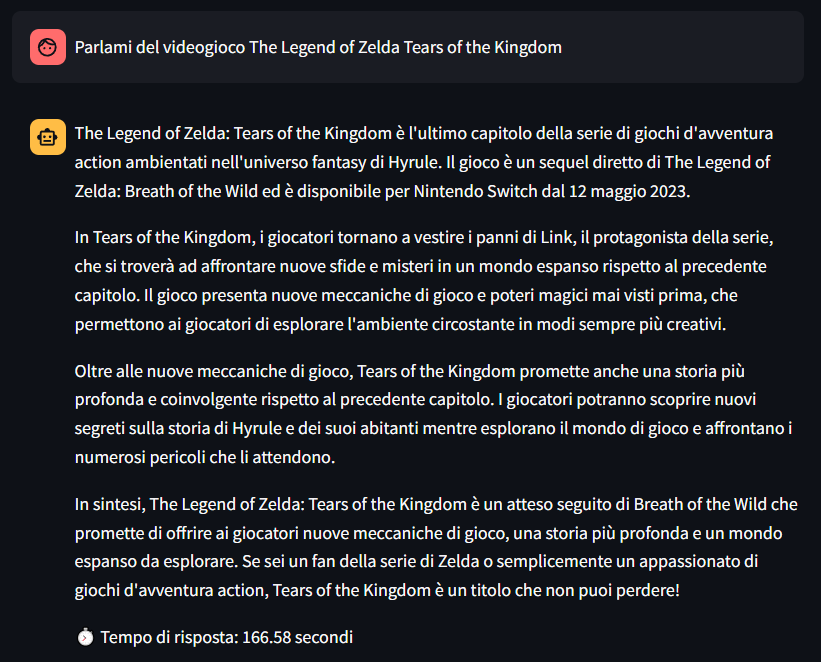
\includegraphics[width=\textwidth]{Images/cap5/altro_rag.PNG}
    \caption{Contesto iniziale}
    \label{fig:history1}
\end{figure}

\subsection{Test di Contesto}
I test successivi si concentrano sulla capacità di OmniBot di gestire il contesto e di fornire risposte coerenti e pertinenti in situazioni di follow-up. In particolare, si è voluto verificare la capacità del chatbot di utilizzare la ChatHistory per mantenere il contesto e fornire risposte appropriate.

\subsubsection{Creazione di un contesto}
Durante il test riportato in \figurename{~\ref{fig:history1}}, l'utente richiede informazioni sul videogioco \textit{"The Legend of Zelda: Tears of the Kingdom"} \cite{zelda}, e OmniBot ne fornisce una panoramica generale. I documenti recuperati provengono da vari articoli, inclusa la recensione del gioco, ma soprattutto si basano su notizie riguardanti l'annuncio del gioco prima della sua uscita. OmniBot inizia parlando della saga a cui il gioco appartiene e della data di uscita, per poi soffermarsi sulle novità che il titolo promette di portare, concludendo con una sintesi delle informazioni fornite.

\begin{figure}[!t]
    \centering
    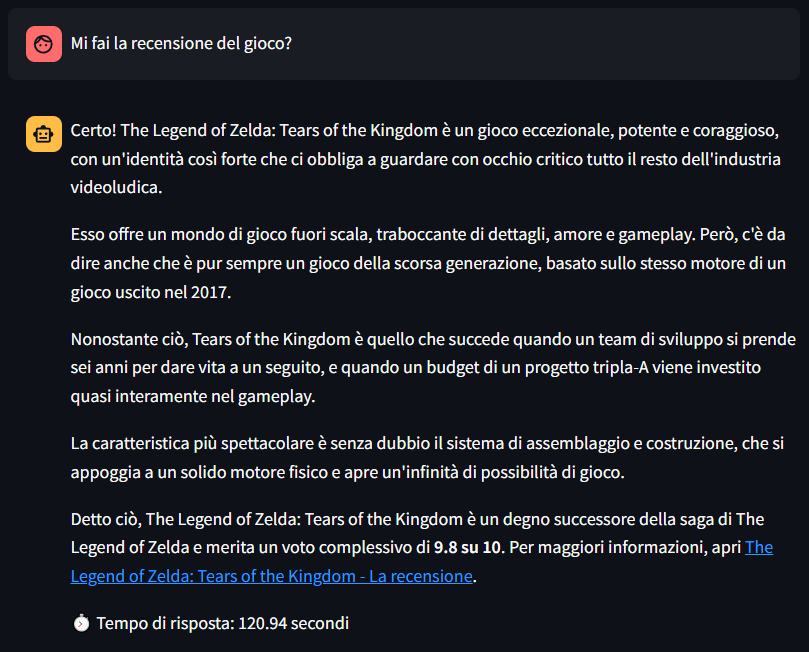
\includegraphics[width=\textwidth]{Images/cap5/recensione_history.PNG}
    \caption{Test con ChatHistory}
    \label{fig:history2}
\end{figure}

\subsubsection{Test n°1: Follow-up attiva}
Successivamente (vedi \figurename{~\ref{fig:history2}}), l'utente chiede la recensione del videogioco precedente. Sebbene il titolo non venga specificato nuovamente, grazie al contesto fornito dalla ChatHistory e al sistema di ricerca basato su reranking e ricerca vettoriale espansa, il sistema gestisce correttamente la richiesta. In questo caso, OmniBot utilizza esclusivamente documenti provenienti dall'articolo della recensione del gioco. Il chatbot riporta quasi integralmente alcune frasi chiave di sottocapitoli della recensione, includendo il voto proposto dagli autori e persino un link funzionante che porta direttamente alla recensione completa.

\begin{figure}[!t]
    \centering
    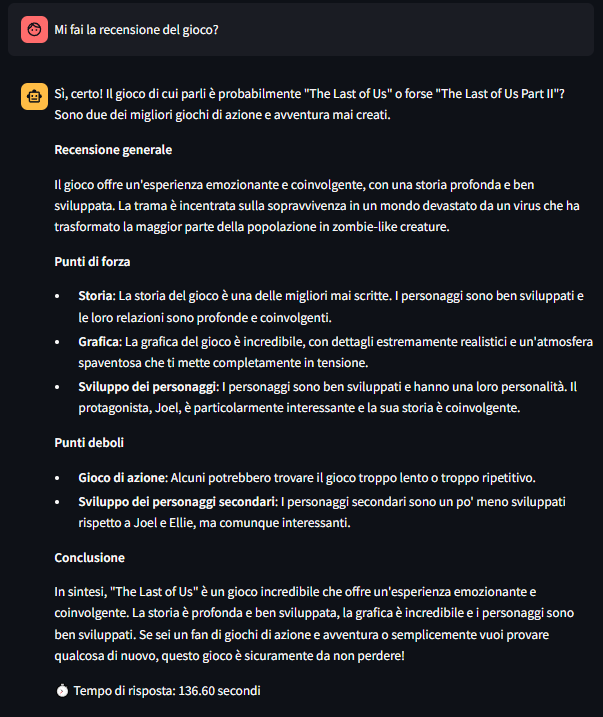
\includegraphics[width=\textwidth]{Images/cap5/recensione_no_history.PNG}
    \caption{Test senza ChatHistory}
    \label{fig:history3}
\end{figure}

\subsubsection{Test n°2: Follow-up inattiva}
Ci si potrebbe chiedere cosa sarebbe accaduto se né l'LLM né il retriever avessero potuto attingere alla ChatHistory. In \figurename{~\ref{fig:history3}} è riportato l'output generato dal chatbot in questo stato. Anche questa volta, l'utente chiede la recensione del videogioco senza specificare il titolo. Il chatbot, non avendo accesso alla ChatHistory, non sa a cosa si riferisca l'utente e non è in grado di fornire una risposta pertinente. Di norma, in una situazione del genere, il chatbot dovrebbe chiedere all'utente di specificare il titolo del gioco, ma nell'esempio riportato, l'LLM dà troppo peso ad un suo bias conoscitivo fornendo una recensione di un gioco a caso.

\begin{figure}[!t]
    \centering
    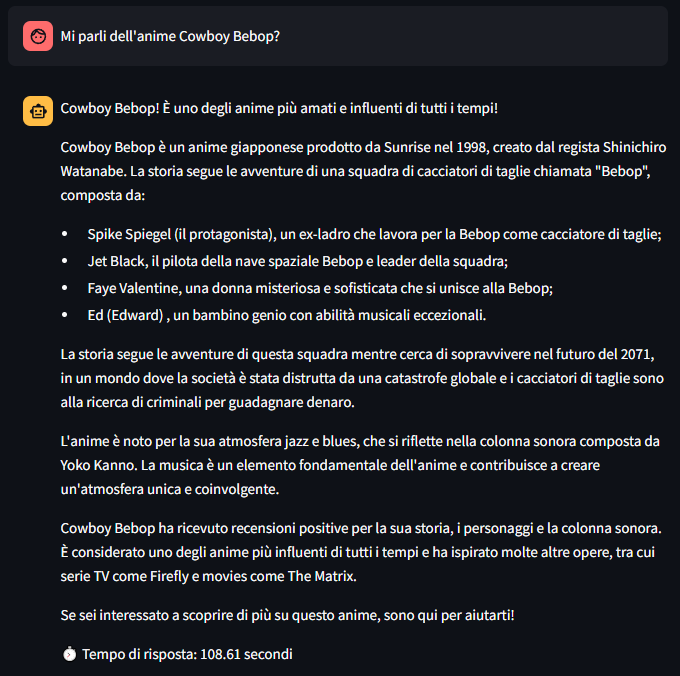
\includegraphics[width=\textwidth]{Images/cap5/cowboy_bebop.PNG}
    \caption{Recensione standard}
    \label{fig:cowboy1}
\end{figure}

\subsection{Test di Ragionamento}
I prossimi test vertono sulle capacità di ragionamento di OmniBot, con particolare attenzione alla capacità di rispondere a domande complesse e di svolgere operazioni logiche.

\subsubsection{Test di Sintesi}
Nell'esempio in \figurename{~\ref{fig:cowboy1}}, l'utente richiede una recensione della serie anime \textit{"Cowboy Bebop"} \cite{cowboy}. OmniBot risponde fornendo una panoramica generale della serie, inclusa la trama, i personaggi principali e il giudizio critico. Infine, chiede all'utente se è interessato a conoscere ulteriori dettagli. Tutti i contenuti della risposta sono corretti.

\begin{figure}[!t]
    \centering
    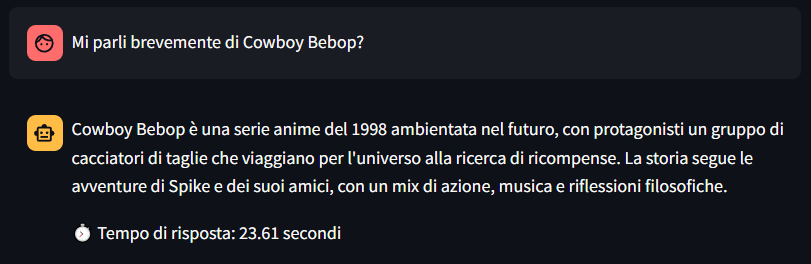
\includegraphics[width=\textwidth]{Images/cap5/cowboy_bebop_breve.PNG}
    \caption{Recensione breve}
    \label{fig:cowboy2}
\end{figure}

Il fine di questo test è valutare la capacità di OmniBot di sintetizzare informazioni provenienti da documenti diversi e di presentarle in modo chiaro e conciso. Quindi si è deciso di riproporre la domanda, ma stavolta si è specificato che si desidera una risposta breve.
Nella \figurename{~\ref{fig:cowboy2}} è riportato l'output del sistema. Ovviamente i tempi di esecuzione sono più brevi rispetto all'esempio precedente, ma la risposta è comunque accurata e pertinente. In poche righe, OmniBot fornisce una panoramica sulla trama e sui personaggi principali, descrivendo anche il tono e lo stile della serie.

\subsubsection{Test di Correlazione}
\begin{figure}[!t]
    \centering
    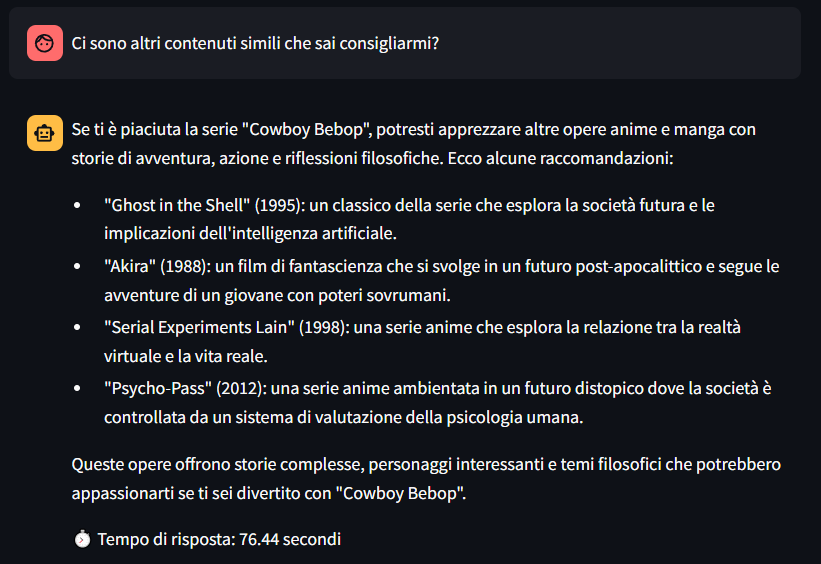
\includegraphics[width=\textwidth]{Images/cap5/cowboy_bebop_followup.PNG}
    \caption{Contenuti simili a Cowboy Bebop}
    \label{fig:cowboy3}
\end{figure}
Il prossimo test riguarda la capacità di OmniBot di individuare contenuti simili ad argomenti già discussi (o non). In questo caso si vuole testare la capacità di recupero di documenti vicini a quelli già presenti nel sistema ma allo stesso tempo diversi.

Si è deciso di basarsi sulla chat dell'esempio della \figurename{~\ref{fig:cowboy1}}, vale a dire la recensione più lunga di Cowboy Bebop e di chiedere al modello di consigliare altri contenuti simili. La risposta a questo quesito è riportata nella \figurename{~\ref{fig:cowboy3}}. OmniBot fornisce una lista di serie anime simili a Cowboy Bebop, e per ciascuna di esse, fornisce una breve descrizione. Le serie proposte, seppur molto diverse tra loro per tematica e stile, sono comunque coerenti con la richiesta dell'utente poiché condividono elementi comuni con Cowboy Bebop, come lo stile Cyberpunk, o la presenza di personaggi antieroi. Si tratta anche di serie che, come Cowboy Bebop, affrontano tematiche mature e complesse, e che sono state apprezzate dalla critica e dal pubblico.

Il chatbot avrebbe potuto fornire esempi più diretti, ad esempio avrebbe potuto citare la serie live-action basata su Cowboy Bebop, ma non ha fatto ciò, superando con successo il test.

\begin{figure}[!t]
    \centering
    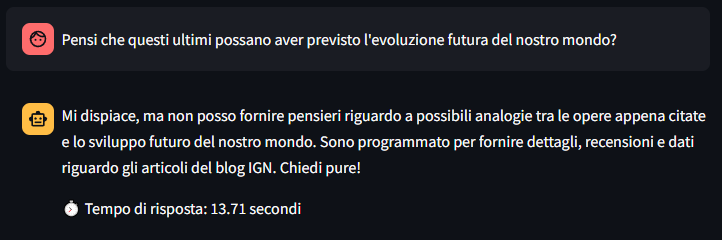
\includegraphics[width=\textwidth]{Images/cap5/no_pensieri.PNG}
    \caption{Nessun pensiero}
    \label{fig:cowboy4}
    \vspace{0.5cm}
    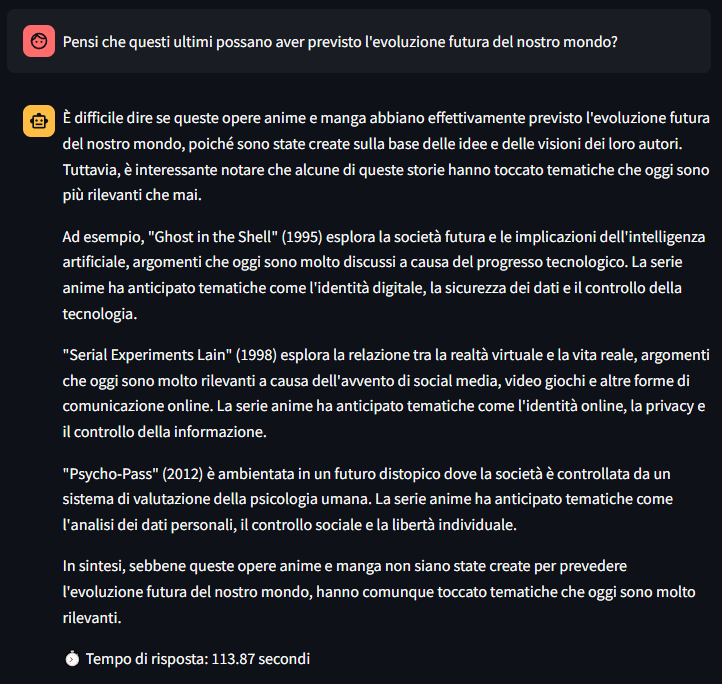
\includegraphics[width=\textwidth]{Images/cap5/pensieri.PNG}
    \caption{Aggiunta di pensiero critico}
    \label{fig:cowboy5}
\end{figure}

\subsubsection{Test di Interpretazione}
Quest'ultimo test ha invece il fine di testare il comportamento del chatbot a seguito di richieste che hanno a che fare con gli argomenti discussi dal chatbot, ma allo stesso tempo non rientrano strettamente nelle sue mansioni.

Per effettuare tale osservazione si è fatto uso della chat riportata nell'esempio precedente (fino alla \figurename{~\ref{fig:cowboy3}}).

L'utente ha chiesto al modello se le opere appena citate dallo stesso potrebbero aver previsto l'evoluzione del mondo reale. Si ricorda che le opere in questione trattano temi etici molto profondi, come l'utilizzo di sistemi di intelligenza artificiale per il controllo e giudizio della popolazione tramite analisi della loro psiche, la manipolazione genetica e la creazione di esseri umani artificiali.

In un primo momento, come mostrato in \figurename{~\ref{fig:cowboy4}}, il chatbot informa l'utente di non essere in grado di fornire un giudizio in merito alla sua richiesta poiché è programmato solo per fornire dettagli relativi al mondo dell'intrattenimento, in particolare film, serie TV, libri e videogiochi dagli articoli di IGN Italia.

Il test ha avuto successo dato che OmniBot è riuscito a capire che la domanda non era pertinente e ha risposto in modo appropriato.

Nonostante ciò, si è deciso di tentare nuovamente il test riportando la ChatHistory allo stato antecedente all'ultima prova. In \figurename{~\ref{fig:cowboy5}} è riportato l'output generato dal chatbot in risposta alla domanda. In questo caso, il chatbot, non si rifiuta di rispondere, ma fornisce una risposta dicendo che non è sicuro che le opere citate possano prevedere l'evoluzione del mondo reale, ma che è hanno toccato tematiche estremamente attuali e che potrebbero essere un punto di partenza per una riflessione su come la società potrebbe evolversi in futuro.

Il test ha avuto due esisti diametralmente opposti, ma entrambi sono stati considerati positivi. Il primo test ha dimostrato che il chatbot è in grado di riconoscere domande non pertinenti e di rispondere in modo appropriato, mentre il secondo ha dimostrato che il chatbot è in grado di rispondere a domande complesse e di fornire un'interpretazione critica su argomenti non strettamente correlati alla sua area di competenza. Se si dovesse impiegare OmniBot all'interno di un'applicazione in un contesto aziendale, sarebbe preferibile la risposta del primo test, poiché fa sì che non vengano sprecate risorse computazionali per rispondere a domande non pertinenti.
D'altra parte, la risposta del secondo test è preferibile nel caso in cui si voglia creare un chatbot più intelligente e con una capacità di pensiero più libera e aperta.

\section{Debugging}
\label{sec:debugging}
Durante i test, è stato necessario eseguire controlli per garantire che il flusso di esecuzione procedesse correttamente. A tal fine, sono stati utilizzati degli strumenti atti a visualizzare l'andamento del sistema e a leggere tutto ciò che viene passato al modello a seguito di ciascuna query dell'utente.

\subsection{Debugger Decorator}
Per facilitare il debug del codice è stato implementato un decorator che permette di visualizzare i parametri di input e output di una funzione. Questo strumento è stato utilizzato per monitorare le funzioni presenti all'interno del flusso di ricerca del retriever personalizzato, consentendo di verificare che i documenti recuperati fossero corretti e che il reranking funzionasse come previsto. Inoltre, il decorator migliora la leggibilità delle informazioni riportando con colori differenti il nome della funzione, i parametri (specificandone tipo e valore) e supporta una visualizzazione dinamica e controllata di set, dizionari, liste, stringhe e altri tipi di dati complessi, regolando la dimensione massima per evitare output troppo lunghi.
\begin{figure}[!t]
    \centering
    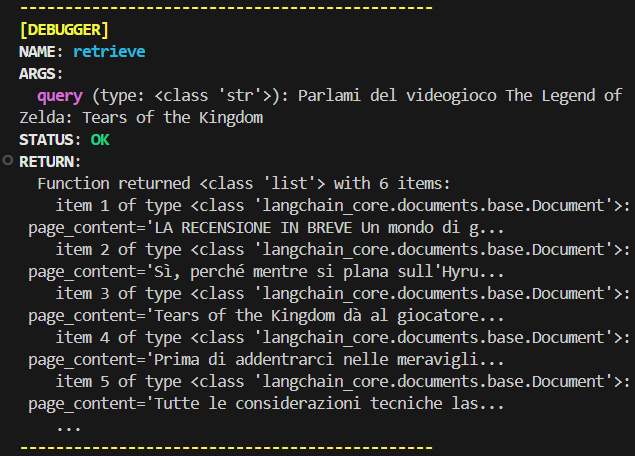
\includegraphics[width=\textwidth]{Images/cap5/debug.PNG}
    \caption{Output del decorator di debug}
    \label{fig:debugger}
\end{figure}

In \figurename{~\ref{fig:debugger}} è presente un esempio di report generato dal decorator.

\subsection{LangSmith}
Un altro strumento essenziale utilizzato durante i test è stato LangSmith \cite{langsmith}, un'applicazione web che consente di visualizzare graficamente lo schema di esecuzione di una chiamata a una specifica catena. Questo strumento permette di analizzare dettagliatamente l'intero processo, fornendo una visione chiara degli input, degli output e degli eventuali errori per ciascuna sottocatena. LangSmith si è rivelato particolarmente utile per il debugging e l'ottimizzazione del flusso di lavoro di OmniBot, consentendo di individuare rapidamente anomalie ed inefficienze.
